\chapter{Special Cases and Restrictions}
\label{chapter:special}

Having proven that \probBook is a hard problem in the previous section,
we now turn to some special instances or variations on \probBook and
either show how they can be solved efficiently or why they remain hard.
This section is the main contribution of this thesis.

One topic we are interested in is how embeddability depends
on the connectivity of the pages. Thus, we deal with both extreme
cases with regards to connectivity in the first two sections: The pages
can either all be connected~(\myref{section:connected}), or ``maximally
disconnected'' without isolated vertices~(\myref{section:matchings}), \ie consisting of perfect disjoint matchings.

We show that the connected case---quite surprisingly---admits a solution
in linear time.
For each page we get a \PQ-tree (see \myref{def:pq}) that stands for the
possible orders of the vertices in a page embedding of this single page.
The solution intersects these sets of orders to decide embeddability. 

In contrast, we are unable to provide an efficient algorithm if the edges of each
page form perfect disjoint matchings. We only manage to prove for this
case that an embeddable graph must be bipartite. Furthermore, we derive---by hand and using a computer---positive bipartite instances and the smallest bipartite counterexamples for all numbers of pages with the
exception of three pages. For three pages we are able to get a smallest counterexample
when two of the matchings form a cycle.

Another interesting restriction we make in \myref{section:trees} is to allow the order of the 
vertices on the spine to only come from the
permutations represented by a fixed \PQ-tree. We present a quadratic time algorithm
for solving the book embedding problem with this restriction if we only allow \Q-trees.
Angelini et.\,al.~\cite{angelini11} showed that a similar restriction is important by reducing \SEFECON~(see page~\pageref{prob:sefecon}) to a book embedding problem
with 2~pages constrained by a \PT-tree.

Finally, in \myref{section:multi_spine} we give a related 
variation on the book embedding problem. We now allow multiple spines~(parallel lines) in the plane
and associate every vertex with a spine the vertex has to be drawn on. 
Additionally, we demand that edges are drawn between consecutive spines, above the
topmost spine or below the bottommost spine. We show that this variation is equivalent to
a special case of the 2-page book embedding problem where the vertex order is constrained
by a \PT-tree, \ie it is indeed related to the problem
of \myref{section:trees}.

While the results we present are mostly independent of each other and small, they
still provide significant insight into the book embedding problem and
\myref{section:trees} is a step towards solving \prob{sefe}. 

\section{Connected Graphs}\label{section:connected}

One approach for solving the book embedding problem is to
determine the
set of valid total orders (permutations) for each of the pages and obtain
the valid book orders by intersecting these sets. Since there are~$n!$ 
permutations on~$n$ vertices, this method is not efficient and even needs super-polynomial space. Indeed, we have
shown in the previous chapter that we cannot expect there to be an efficient algorithm.

We know that cyclic shifts and mirror images do not matter. Considering this, 
we can encode the possible valid orders more efficiently by 
only storing one symmetric order in place of $2n$ total orders. However, this
is still not sufficient for efficiently solving the book embedding problem.
Are there better encodings that make the algorithm
feasible, at least for special graphs?

As a matter of fact, there are. In this section we see that the valid total orders can be encoded
very efficiently using \PQ-trees if the pages are connected---the first special case of~\probBook we consider. Furthermore, \PQ-trees on the
same vertices can also be efficiently \emph{intersected}, \ie we can efficiently 
get a \PQ-tree representing~$\pi(T_1) \cap \pi(T_2)$ from two \PQ-trees $T_1$ and~$T_2$ on the same leaves.

\newProb{\probBookConnected}{A vertex set~$V$ and edge sets~$E_1,\dotsc,E_k \subseteq \binom{V}{2}$ such
that the graphs~$(V, E_i)$ are connected for~$i \in \range{k}$.}{Is there
a book embedding of $(V, E_1),\dotsc, (V,E_k)$?}

%TODO
%
%We can reinterpret a \PQ-tree to represent a set of cyclic orders instead of linear order.
%To do this, add a new root $p$~whose only neighbour is the original root of the tree. In all possibilities
%for flipping the tree's \PT- and \Q-nodes, define the corresponding circular order as follows: Start at~$p$, go along the
%linear order of the tree and end at~$p$. If we disregard~$p$ in this order, we get a circular order on
%the original leaves. That is, we can map a linear order on the
%leaves to a cyclic order by
%writing the leaves in the linear order on a cycle.
%Since, for example, 12345 and~23451 both yield the
%same cyclic order, this map need not be injective.

\paragraph{Planarity testing using \PQ-trees}

There are several planarity testing algorithms that represent the possible planar
embeddings using \PQ-trees. A high-level scheme for these methods is
described by Haeupler and Tarjan~\cite{Haeupler08}. It can be adapted to give
all valid orders of a page embedding as we show below.

We first briefly describe this scheme. 
It embeds the graph $G$~vertex by vertex. At each step
we store the set of possible partial planar embeddings where some subset
of the vertices has already been embedded. 

The edges that have exactly 
one embedded endpoint at a step are \emph{half-embedded}. If the non-embedded
vertices form a connected graph at each step, the half-embedded edges must lie on a common face
that we can without loss of generality assume to be the outer face, \ie all the already embedded vertices incident to half-embedded edges are on the boundary of the outer face. 

That the non-embedded vertices form a connected graph can be guaranteed
by choosing a leaf-to-root order in any fixed spanning tree of the connected graph~$G$. The possible
partial embeddings can then be represented by the order of their half-embedded edges
around the outside of their component.
 
It can be shown that these orders are given by a \PQ-tree for every component of the subgraph
induced by the embedded vertices. For a more detailed explanation consult the
paper by Haeupler and Tarjan~\cite{Haeupler08}. They also show how to implement the
scheme in linear time.

\paragraph{Representing book embeddings using \PQ-trees}

This is not yet what we want. A page embedding is an outerplanar embedding and not a planar embedding.
Thus, we have to modify the planarity algorithm slightly. We build the connected graph $\widetilde{G}$ by
adding a new vertex~$r$ to~$G$ that is adjacent to every vertex in~$V(G)$. In \myref{ch:preliminaries} we noted the
fact that~$G$ is outerplanar if and only if $\widetilde{G}$ is planar. Furthermore, by removing~$r$
from a planar embedding of~$\widetilde{G}$ we get an outerplanar embedding of~$G$.

\begin{figure}[\placement]
    \centering
    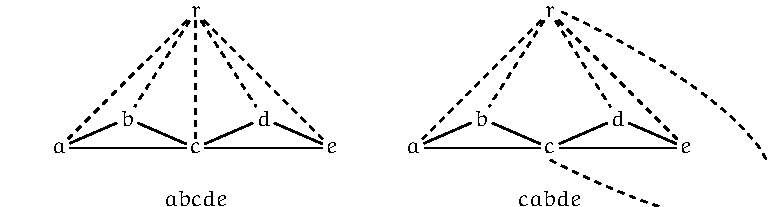
\includegraphics[scale=.9]{figures/t_subtle}
    \caption[Outerplanar embedding representing different symmetric orders]{The outerplanar embedding  
    represents the vertex orders in both $[abcde]$ and~$[cabde]$. The symmetric orders $[abcde]$ and~$[cabde]$ correspond to different edge orders around~$r$ in the extended graph.}
    \label{figure:subtle}
\end{figure}
    
Now we choose~$r$ as last vertex in the leaf-to-root order of the planarity algorithm.
Since $G$~is connected, the scheme above yields a single \PQ-tree~$T$ representing all
extendible planar embeddings of~$G$ (as possible orders of the half-embedded edges~$\{r, v\}$ for~$v\in V(G)$)  at its penultimate step. By the argument above, every such embedding
is outerplanar. Also, $T$~not only gives the orders of the half-embedded edges
but all vertices of~$G$ since~$r$ is adjacent to every other vertex, \ie every vertex of~$G$ is 
the endpoint of exactly one half-embedded edge. 

A subtle distinction is still noteworthy, although it does not present any problems
for the algorithm. When
walking around the outer boundary of an outerplanar embedding in clockwise or counter-clockwise
direction, we can meet a vertex twice. Thus, the outerplanar embedding in \myref{figure:subtle},
for example, can yield the total orders in both $[abcde]$ and~$[cabde]$; yet these orders belong
to different planar embeddings of the extended graph.

In conclusion, there is a \PQ-tree from which we can read all valid outerplanar embeddings (page embeddings). 
This \PQ-tree can be computed in linear time as shown by Haeupler and Tarjan~\cite{Haeupler08}.
%For~$C_4$ this is illustrated in \myref{figure:connected}.

\begin{lemma}\label{lemma:one-page}
Let~$G = (V, E)$ be a connected graph. Then we can compute a \PQ-tree representing all valid
orders of the vertices~$V$ in a page embedding of~$G$ in $\OO\bigl(|V|\bigr)$~time.
\end{lemma}

To get the set of valid book orders, all that remains to be done is to intersect the
\PQ-trees we get. Say we want to intersect the \PQ-trees~$S$ and~$T$ on the same leaves. Let~$v$
be an inner node of~$S$ and~$e$ one of its incident edges going to a child~$w$ of~$v$.
Then the leaves $C(w)$~that have~$w$ as ancestor appear consecutively in any order $\pi \in \pi(S)$.
Additionally, if~$v$ is a \Q-node and $e'$ is a consecutive edge of~$e$ going from~$v$ to~$w'$, then the
leaves $C(w) \cup C(w')$ also appear consecutively in any $\pi \in \pi(S)$. On the other hand,
any order fulfilling these constraints is in~$\pi(S)$. That is, we can get a tree
representing $\pi(S) \cap \pi(T)$ by applying the reductions just described to the tree~$T$.
A trivial implementation of this approach would need a quadratic number of reductions, but Booth described in his Ph.\,D. thesis~\cite{Booth75}
how to reduce the cost of intersection to linear time.

Now that we are able to intersect \PQ-trees, we can summarise the linear-time solution
of \probBookConnected.

\begin{theorem}
\probBookConnected can be solved in linear time.
\label{theorem:connected}
\end{theorem}
\begin{myproof}
Let~$(V, E_1,\dotsc, E_k)$ be the \probBookConnected instance.
First construct the $k$ \PQ-trees~$T_1,\dotsc, T_k$ representing all valid page
embeddings of the corresponding graphs~$(V, E_1), \dotsc, (V,E_k)$, each in~$\OO\bigl(|V|\bigr)$. Then consecutively
intersect $T_1$ with $T_2,\dotsc, T_k$ using time~$\OO\bigl((k - 1)|V|\bigr)$, yielding the
\PQ-tree~$T$ representing all valid solutions of the instance. The instance
possesses a solution if and only if~$T \ne \varepsilon$, which can be decided in constant time.
All in all, we need $\OO\bigl(k|V|\bigr)$~time.
\end{myproof}

\paragraph{Outlook}

When the graphs on the pages are not connected, we also get \PQ-trees for the valid orders of each of their components. That is, we have a set of \PQ-trees and must decide whether
they possess a common order in order to solve the book embedding problem. The hurdle is that the trees do not need to have the same leaves. 

Bl\"asius and Rutter~\cite{Blasius11} considered a more general variant of this \PQ-tree intersection problem, called \probPQ. They showed the
\NP-completeness of \probPQ for an unbounded number of trees. 
%As noted in \myref{section:np-complete}, we, similarly, only showed that \probBook
%is \NP-complete when the number of pages is unbounded. 
Investigating restrictions of \probPQ
may help us deal with the book embedding problem, but we are not sure how.
%By the reduction above, we can
%improve this to a constant number of pages if we manage to prove the \NP-completeness
%of \probPQ for a constant number of trees. Therefore, investigating \probPQ is one approach for extending
%our results, but it is---in our opinion---not promising since
%\probPQ is not a problem of significantly simpler form than \probBook.
\section{Disjoint perfect matchings}

\begin{frame}{Disjoint perfect matchings as pages}

%Take disjoint perfect matchings as pages.
\newProb{\probMatching}
{Disjoint perfect matchings $E_1,\dotsc, E_k$ on a vertex
set $V$.}{Is there a book embedding of $(V, E_i)$?}

\begin{theorem}
Necessary: $G := (V, E_1 \cup \dotsb \cup E_k)$ is bipartite.
\end{theorem}

\begin{overprint}
\onslide<1>
\begin{itemize}
\item Even number of vertices between adjacent vertices in valid order
\begin{figure}
\centering

\resizebox{0.6\textwidth}{!}{
\begin{tikzpicture}
\node (v) {v};
\node[right of=v,node distance=7em] (nw) {$n_i(w)$};
\node[right of=nw,node distance=7em] (w) {$w$};
\node[right of=w,node distance=7em] (nv) {$n_i(v)$};

\draw (v) edge[bend left] (nv);
\draw (nw) edge[bend left] (w);

/* v to n1 */
\draw[decoration={brace},decorate,thick] ($ (nv) + (-1.2em, -1em) $) -- ($ (v) + (0.5em,-1em) $);
\node[text centered] at ($ 0.5*($(nv) + (v)$) + (-0.25em, -2em) $) {even};

\node[text centered] at ($ 0.5*($(v) + (nw)$) + (0.25em, 0)$) {\dots};
\node[text centered] at ($ 0.5*($(nw) + (w)$) + (0.25em, 0)$) {\dots};
\node[text centered] at ($ 0.5*($(w) + (nv)$) + (0.25em, 0)$) {\dots};
\end{tikzpicture}
}
\end{figure}
\end{itemize}

\onslide<2>
\begin{itemize}
\item Even number of vertices between adjacent vertices in valid order
\item[$\Rightarrow$] Vertices with even and odd indexes form bipartition
\end{itemize}
\end{overprint}

\end{frame}

\begin{frame}{Bipartite examples}
\begin{figure}[\placement]
\centering

\scalebox{1.3}{%
\begin{tikzpicture}

\node (l1) {{\relscale{0.5}$l_0$}};
\node[right of=l1,node distance=6em] (r1) {{\relscale{0.5}$r_0$}};
\node[below of=l1] (l2) {{\relscale{0.5}$l_1$}};
\node[right of=l2,node distance=6em] (r2) {{\relscale{0.5}$r_1$}};
\node[below of=l2] (l3) {{\relscale{0.5}$l_2$}};
\node[right of=l3,node distance=6em] (r3) {{\relscale{0.5}$r_2$}};
\node[below of=l3] (l4) {{\relscale{0.5}$l_3$}};
\node[right of=l4,node distance=6em] (r4) {{\relscale{0.5}$r_3$}};

\draw (l1) edge (r1);
\draw (l2) edge (r2);
\draw (l3) edge (r3);
\draw (l4) edge (r4);
\draw[edge1] (l1) edge (r2);
\draw[edge1] (l2) edge (r3);
\draw[edge1] (l3) edge (r4);
\draw[edge1] (l4) edge (r1);
\draw[edge2] (l1) edge (r3);
\draw[edge2] (l2) edge (r4);
\draw[edge2] (l3) edge (r1);
\draw[edge2] (l4) edge (r2);
\draw[edge3] (l1) edge (r4);
\draw[edge3] (l2) edge (r1);
\draw[edge3] (l3) edge (r2);
\draw[edge3] (l4) edge (r3);
\end{tikzpicture}}
\end{figure}

$k$ pages: Take the partition $E_i := \bigl\{\{l_j, r_{(j + i)\bmod{k}}\}: j \in \range{k-1}\bigr\}$ of $K_{k,k}$ 
\end{frame}

\begin{frame}{Bipartite counterexamples}
\begin{figure}[\placement]
\centering

\scalebox{1.3}{%
\begin{tikzpicture}

\node (l1) {{\relscale{0.5}$l_1$}};
\node[right of=l1,node distance=6em] (r1) {{\relscale{0.5}$r_1$}};
\node[below of=l1] (l2) {{\relscale{0.5}$l_2$}};
\node[right of=l2,node distance=6em] (r2) {{\relscale{0.5}$r_2$}};
\node[below of=l2] (l3) {{\relscale{0.5}$l_3$}};
\node[right of=l3,node distance=6em] (r3) {{\relscale{0.5}$r_3$}};
\node[below of=l3] (l4) {{\relscale{0.5}$l_4$}};
\node[right of=l4,node distance=6em] (r4) {{\relscale{0.5}$r_4$}};

\draw (l1) edge (r1);
\draw (l2) edge (r2);
\draw (l3) edge (r3);
\draw (l4) edge (r4);
\draw[edge1] (l1) edge (r2);
\draw[edge1] (l2) edge (r1);
\draw[edge1] (l3) edge (r4);
\draw[edge1] (l4) edge (r3);
\draw[edge2] (l1) edge (r3);
\draw[edge2] (l3) edge (r1);
\draw[edge2] (l2) edge (r4);
\draw[edge2] (l4) edge (r2);
\draw[edge3] (l1) edge (r4);
\draw[edge3] (l4) edge (r1);
\draw[edge3] (l2) edge (r3);
\draw[edge3] (l3) edge (r2);
\end{tikzpicture}}
\end{figure}

$k \geq 4$ pages: Partition $K_{k,k}$ into disjoint perfect matchings that contain
this counterexample
\end{frame}

\begin{frame}{Bipartite counterexample for three pages}
Smallest counterexample where two of the matchings form a cycle\vspace{-1em}
\begin{figure}[\placement]
\centering
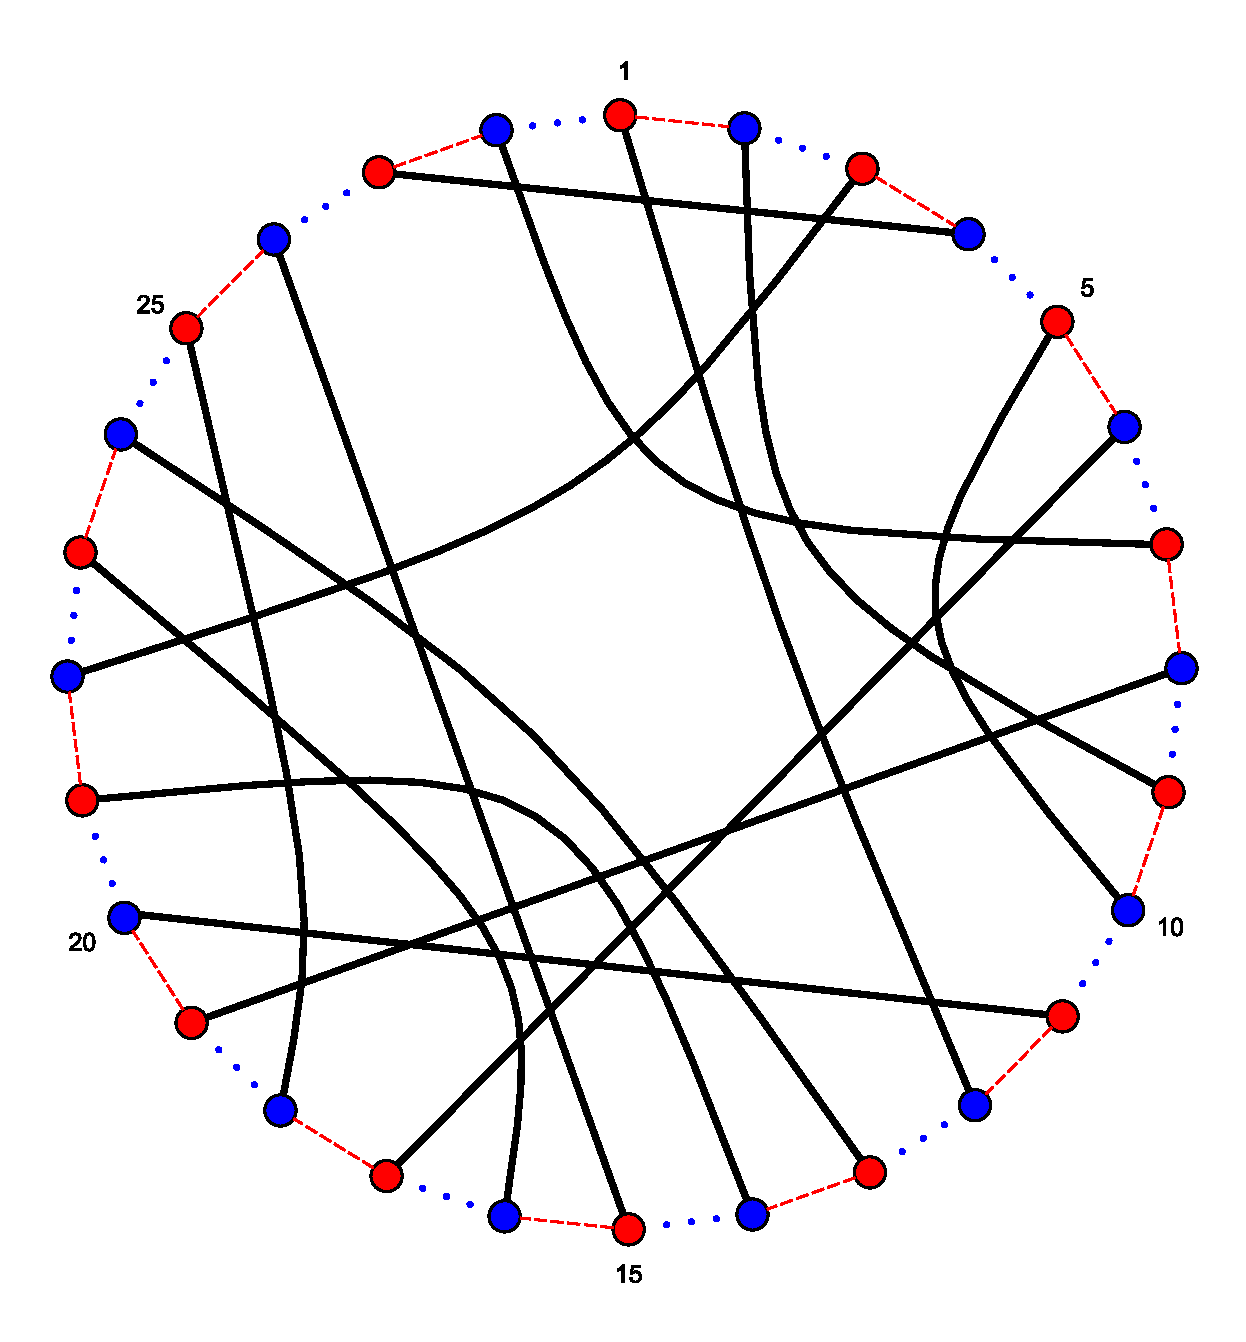
\includegraphics[width=0.5\textwidth]{../thesis/figures/two_cycles.eps}
\end{figure}
\vspace{-1em} Smallest unrestricted counterexample: $20 \leq n \leq 28$
\end{frame}

\resultFrame{4}
\section{\PQ-tree on the Vertices}
\label{section:trees}

\noindent 

Besides demanding that pages have a special structure, as we have
done in the preceding sections, we may
restrict the order of the vertices to a subset
of the symmetric group~$S_n$ that we can, hopefully, work with more easily. 

Angelini et.\,al.~\cite{angelini11} showed that \SEFECON~(see page~\pageref{prob:sefecon}) can be reduced to a 2-page embedding problem where the vertex order comes from a \PT-tree.

For this reason it is useful to restrict the permutations with \PQ-trees. That is, we do
the very opposite of \myref{section:connected} and start with a \PQ-tree
instead of getting a tree that represents the possible book embeddings.

\begin{figure}[\placement]\centering
    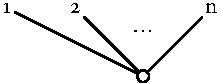
\includegraphics{figures/t_pq-all}
    \caption[\PQ-tree that represents all permutations]{A \PQ-tree that represents all permutations of $\range{n}$.}
    \label{figure:pq-all}
\end{figure}

A general~\PQ-tree does not really help
since the \PQ-tree in \myref{figure:pq-all} (a single \PT-node) represents all permutations of $\range{n}$,
\ie the problem does not get easier.

Thus, we have to narrow down the possible permutations even more. In this section we only consider
\Q-trees and show that \probQTree, which is \probBook restricted to~\Q-trees,
can be solved in quadratic time. In order to do this, we provide a reduction of the problem to~\probTwoSat, the problem of checking a 2-CNF formula for satisfiability. 
The \probTwoSat problem is solvable in linear time as first shown by Krom~\cite{Krom67}.

\newProb{\probQTree}{A \probBook instance $I$ with vertices $V$ and a \Q-tree~$T$ with leaves~$V$.}{Is there a total order $<\,\in \pi(T)$ solving $I$?}
\newProb{\probPTree}{A \probBook instance $I$ with vertices $V$ and a \PT-tree~$T$ with leaves~$V$.}{Is there a total order $<\,\in \pi(T)$ solving $I$?}
\newProb{\probTwoSat}{A 2-\CNF Boolean formula \bool{f}.}{Is~\bool{f} satisfiable?}

\Q-Trees are exactly the wrong type of trees
compared to the reformulation of the \SEFECON problem by Angelini et.\,al.~\cite{angelini11} since \Q-nodes vastly restrict the possible
permutations and are significantly easier to handle than \PT~nodes. This
section, therefore, only solves \SEFECON if the \PT-tree of the equivalent \probPTree instance is also a \Q-tree, \ie if the \PT-tree is a binary tree.

We first investigate what possible configurations of the leaves the book constraints 
lead to when we take the \Q-tree~$T$ into account. Then we show how these configurations
can be expressed with a 2-\CNF formula.

\paragraph{Possible configurations resulting from a book constraint}

\begin{figure}[\placement]\centering
    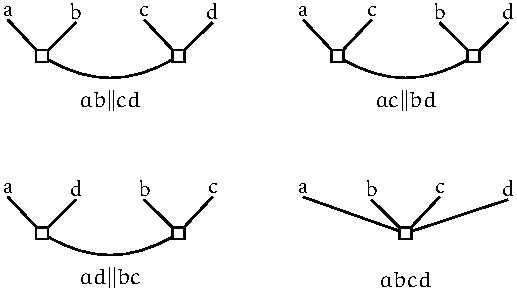
\includegraphics{figures/t_topo1}
    \caption[Topologies of four leaves]{The possible topologies of four leaves $a, b, c, d$ in a tree.}
    \label{figure:topo1}
\end{figure}


We first show that the book embedding restrictions for two edges $\{a, b\}$ and $\{c, d\}$
can be translated directly to restrictions on the $Q$-tree.
Before we start with this translation, however, we list some conventions. The \Q-tree is called $T$ and has leaves~$V$. Furthermore, let $t(M)$ be the smallest subtree of~$T$ containing~$M$ and let~$r(M)$ be its root for any~$M \subseteq V$.
Also remember that we assumed  in \myref{section:total-ordering} that any two edges we consider the book constraint for are independent.

%Consider the tree~$t(M)$ for~$M := \{a, b, c, d\}$.

We want to distinguish cases based on which two leaves in~$M := \{a, b, c, d\}$ can be separated from the others. These possible \emph{topologies of $M$ in~$T$} are depicted in \myref{figure:topo1}.
For example, we have~$ab||cd$ if there is an edge~$e \in E(T)$ such that $a$ and~$b$ are
in one component of~$T \setminus e$ while $c$ and~$d$ are in the other component, \ie
$a$ and~$b$ can be separated from $c$ and~$d$.
The topologies for $ac||bd$ and~$ad||bc$ are defined analogously. If no two vertices in~$M$ can be separated from the other
two (all pairs of vertices in~$M$ have the same lowest common ancestor) we say that the topology~$abcd$ occurs. 

%Thus, $t(M)$ has one of the trees in \myref{figure:topo1} as a
%topological minor, \ie the leaves $a$, $b$, $c$ and $d$ can appear
%in only a small number topological configurations. (Note that we do not take into consideration that the tree is rooted and ordered.) We call these configurations ``topologies'' below.

Depending on which of the topologies occurs, we can map the constraint from \myref{lemma:constraints} to a Boolean formula on the order~$<$ of the vertices~$V$.

\paragraph{Case 1: ab||cd}

Since $\{a, b\}$ and $\{c, d\}$ are in disjoint subtrees and the vertices of
a subtree are consecutive in every permutation $\pi(T)$, all tree orders
fulfil the book constraint. Thus, the constraint is mapped to the Boolean expression \bool{true}.

\paragraph{Case 2: ac||bd}

\begin{figure}\centering
    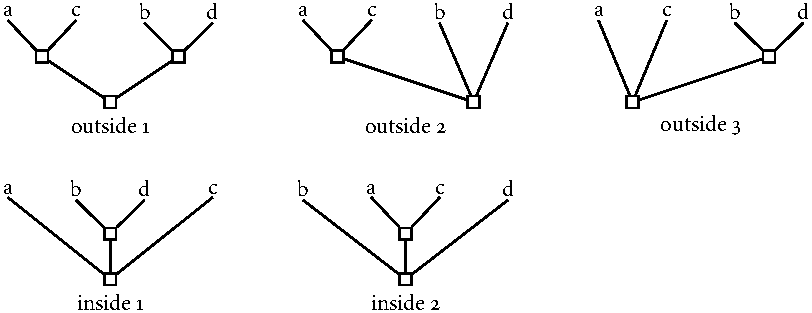
\includegraphics[scale=.9]{figures/t_order_ab_cd}
    \caption[Trees for $ac||bd$]{The possible trees corresponding to $ac||bd$.}
    \label{figure:order_ab_cd}
\end{figure}
\begin{figure}\centering
    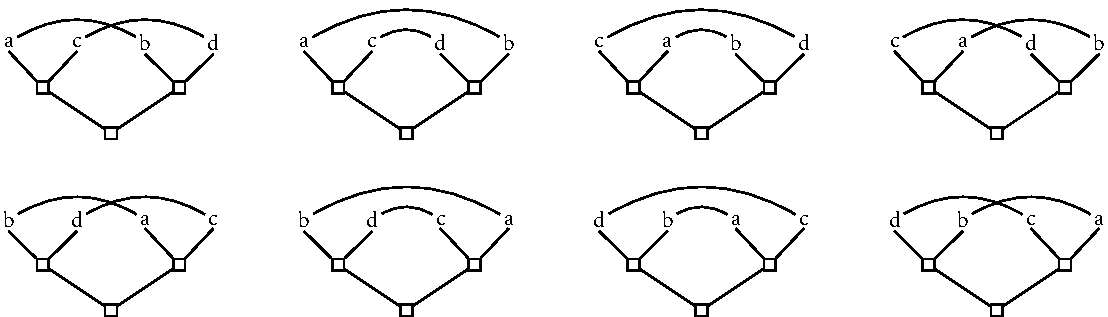
\includegraphics[width=\textwidth]{figures/t_topo_ac_bd}
    \caption[Outside 1 tree orders]{The tree orders for the case outside 1.}
    \label{figure:topo_ac_bd}
\end{figure}
\begin{figure}\centering
    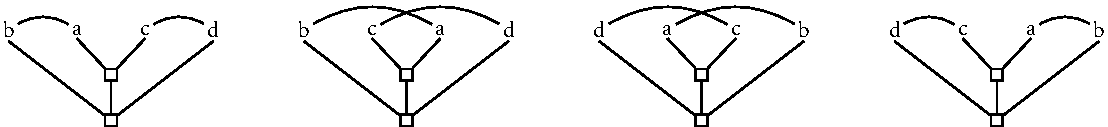
\includegraphics[width=\textwidth]{figures/t_topo_b_ac_d}
    \caption[Inside 1 tree orders]{The tree orders for the case inside 1.}
    \label{figure:topo_b_ac_d}
\end{figure}

In this case we search through the possible trees to determine the resulting
\probTwoSat formula. To do this systematically, we have to take into account that~$T$ is ordered and rooted and determine what the tree can look like. 

Thus, we further split this case into sub-cases based on whether the vertices $a$ and~$c$ are between $b$ and~$d$ (inside), $b$ and~$d$ are between $a$ and~$c$ (inside) or no two vertices in~$M$ are between the vertices they are separated from (outside). Note that $a$ and~$c$ are between $b$ and~$d$
for all orders in~$\pi(T)$ if they are between $b$ and~$d$ for one order in~$\pi(T)$ since~$T$
is a \Q-tree.

In the outside case, the
possible permutations also depend on how the roots of the subtrees $t(a, c)$ and $t(b, d)$ are related,
\ie whether one appears as a child of the other. The possible tree structures are depicted
in \myref{figure:order_ab_cd}.  
%We especially need not fix any portion of the order.

For each tree, we can exhaustively search through the orders of the leaves~$M$ the tree permits. For the 
case outside~1 these orders are portrayed in \myref{figure:topo_ac_bd}. We observe that the
valid orders are exactly the orders with $a < c \Leftrightarrow d < b$. The other two outside
cases can be handled similarly. Both of them again yield $a < c \Leftrightarrow d < b$.

For the inside cases we do the same. The possible orders of the case inside~1 are depicted in \myref{figure:topo_b_ac_d}. We can infer the
inverse $a < c \Leftrightarrow b < d$ for both inside cases. 

\paragraph{Case 3: ad||bc}

As in case~2, we either get $a < d \Leftrightarrow b < c$ or
$a < d \Leftrightarrow c < b$.

\paragraph{Case 4: abcd}

Let~$r$ be the common root $r(a, b, c, d)$ of $M := \{a, b, c, d\}$. The tree~$T$
represents two permutations of $M$ since the children of the \Q-node~$r$ can
only be reversed. If the book constraint is valid in a permutation of~$M$, it is also valid in the
mirror image of the permutation. Therefore, the book constraint may be valid in none or both of the two possible permutations. That is, we get either \bool{true} or
\bool{false} as constraint.

\paragraph{Mapping \probBook to \probTwoSat}

We now show how the resulting Boolean expressions can be mapped to \probTwoSat formulae.
To do so we fix a reference orientation of the inner nodes of~$T$.
For each $\pi \in \pi(T)$ and every inner node $v$ in $T$, we can say whether
we got $\pi$ as a permutation in~$\pi(T)$ by giving~$v$ the reference orientation or not.
Introduce a Boolean variable $o_v$ that stands for~$v$ being in reference orientation.

By the construction above, a book constraint for two edges yields one of the following Boolean expressions dependent on the structure of~$T$.

\begin{enumerate}
  \item A trivial expression \bool{true} or \bool{false}. (from cases~1 and~4)
  \item A fixed order of two leaves $v$ and~$w$ which is the same
  as fixing the order of their root~$r := r(v, w)$. Thus, we get
  $o_r$ or $\lnot o_r$. (from case~4)
  \item A connection between the orders of the leaves $a$, $b$ and $c$, $d$
  that are located in disjoint subtrees. This is the same as tying the
  orders of the roots $r := r(a, b)$ and $s := r(c, d)$ together.
  We get either $o_r \Leftrightarrow o_s \equiv (\lnot o_r \lor o_s) \land (\lnot o_s \lor o_r)$
  or $o_r \Leftrightarrow \lnot o_s \equiv (\lnot o_r \lor \lnot o_s) \land (o_s \lor o_r)$. (from cases~2 and~3)
\end{enumerate}

Thus, we can reduce \probQTree to determining whether a set of 2-\CNF expressions
is consistent with a \Q-tree structure. But since the inner nodes of a \Q-tree can be flipped completely independently of each other, the consistency with the \Q-tree structure does not
impose any extra restrictions. That is, \probQTree can be mapped to checking
a \probTwoSat formula for consistency (satisfiability).


%\newProb{\probQTreeSat}{A \Q-tree $T$ and a 2-\CNF expression $m$ on $\{o_v\colon \text{$v$ 
%is inner node of $T$}\}$ with $o_v$~signifying that the node~$v$ is ordered as in the initial tree.}{Is there a permutation in~$\pi(T)$ where~$m$ is satisfied?}

We now see how the reduction from \probQTree to \probTwoSat above can be 
implemented in qua\-dratic time.

\begin{lemma}
\label{lemma:q-tree-redux}
\probQTree can be reduced to \probTwoSat in quadratic time.
%A $\probQTree$~instance  can be reduced
%to a $\probTwoSat$ instance in $\OO\bigl(|T| + |E_1|^2 + \dotsb + |E_k|^2\bigr)$~time.
\end{lemma}
\begin{myproof}
Let $\bigl((V, E_1),\dotsc, (V, E_k), T\bigr)$ be an instance of $\probQTree$.
We can map the book constraints for each pair $e_1, e_2 \in E_i$ of edges for all
$i \in \range{k}$ to a 2-\CNF formula with the construction above.

Let's investigate how this can be done efficiently. Our goal is
to map each book constraint resulting from a pair of edges to a 2-\CNF formula in constant
time after a linear time precomputation. 

We assume $V = \range{n}$ and that each inner node of the tree~$T$ 
contains a pointer to its parent and an (ordered) list of its children.
Furthermore, let~$r$ be the root of~$T$.

%\begin{Ualgorithm}[\placement]
%\caption{Class for rooted, ordered trees}\label{alg:tree}
%\DontPrintSemicolon
%
%\SetKwFor{Class}{class}{}
%
%\SetKwFunction{Tree}{Tree}
%\SetKwFunction{PTree}{Pointer to Tree}
%\SetKwFunction{VTree}{Vector of pointers to Tree}
%\SetKwFunction{MyInt}{Integer}
%
%\Class{\Tree}{parent: \PTree\;children: \VTree}
%\end{Ualgorithm}

To determine the topology of a quadruple of leaves, we need to know
the lowest common ancestor of certain pairs of nodes and their initial order.

The first problem has been studied extensively. Harel and Tarjan~\cite{Harel84} showed
the surprising result that lowest common ancestor queries can be answered in constant
time after a linear time precomputation, although their algorithm was too complicated to be implemented
effectively. Farach and Colton~\cite{Farach00} presented a far simpler variant of this
algorithm that is used in practice. We assume in the following that the precomputation has 
been done and that \algoFont{LCA($x$, $y$)} gives the lowest common ancestor of~$x$ and~$y$ in~$\OO(1)$ time.

For the second problem, we can precompute the index array~\algoFont{idx} of~$V$ that maps each
leaf~$V$ to its index in the reference orientation of~$T$. This can be accomplished in linear time by a simple depth-first search. 

%At each step,
%we know the index the leaves in the current subtree start with. We recurse on the children
%of the current node in order and update the starting index accordingly. When we arrive at a
%leaf, we know that its index is the current starting index, which is given as a parameter. The initial
%call is~\algoFont{ComputeIndex$(r, 1)$}.
%
%\begin{Ualgorithm}[\placement]
%\caption[Computing the index array]{Computing the index array: \algoFont{ComputeIndex}}\label{alg:index}
%
%\SetKwFunction{Tree}{Tree}
%\SetKwFunction{ComputeIndex}{ComputeIndex}
%\SetKwFunction{size}{size}
%\SetKwFunction{content}{idx}
%\SetKwFunction{children}{children}
%
%\SetKwData{T}{T}
%\SetKwData{firstIdx}{s}
%\SetKwData{lastIdx}{e}
%\SetKwData{idx}{idx}
%\SetKwData{mycnt}{i}
%
%\KwIn{Tree $T$, starting index $s$}
%\KwOut{Ending index $e$}
%
%\BlankLine
%\tcp{Is $T$ leaf?}
%\If{$\T.\children.\size = 0$}{
%$\lastIdx \leftarrow \firstIdx$ \;
%$\idx[\T.\content] \leftarrow \firstIdx$
%}
%\Else {
%	\tcp{Recurse and update indexes}
%	\For{$\mycnt \leftarrow 1$ to $\T.\children.\size$}{
%		$\firstIdx \leftarrow \ComputeIndex(\T[\mycnt], \firstIdx) + 1$
%	}
%}
%\end{Ualgorithm}

Before we begin with the actual translation, we need another helper function \algoFont{Leaf-Order($a$,$b$)} that translates a statement
of the form~$a < b$ for leaves $a, b \in V$ into a literal on the variable~$o_r$ 
where $r = \algoFont{LCA}(a, b)$. If $\algoFont{idx[a]} < \algoFont{idx[b]}$, then~$r$ has reference orientation and the result is~$o_r$. Otherwise, the result is~$\lnot o_r$. This decision can obviously
can be made in $\OO(1)$~time.

%\begin{Ualgorithm}[\placement]
%\caption[Literal for leaf order]{A literal for a given leaf order: $\algoFont{Leaf-Order}$}\label{alg:lca}
%
%\KwIn{Leaves $a, b \in V$}
%\KwOut{A Boolean formula representing $a < b$}
%
%\SetKwFunction{LCA}{LCA}
%
%\SetKwData{firstPar}{a}
%\SetKwData{secondPar}{b}
%\SetKwData{idx}{idx}
%
%\BlankLine
%$r \leftarrow \LCA(\firstPar, \secondPar)$ \;
%\If{$\idx[\firstPar] < \idx[\secondPar]$}{
%	\KwRet $o_r$
%}
%\Else{
%	\KwRet $\lnot o_r$
%}
%\end{Ualgorithm}

We now have everything we need to translate book constraints into
Boolean formulae. The direct formalisation of the construction
above is given in \myref{alg:translate}. It returns
a Boolean formula for a pair of edges $\{a, b\}$ and~$\{c, d\}$
in~$\OO(1)$. Note that we can test whether the order~\algoFont{idx} fulfils
the book constraint in line~9 in~$\OO(1)$ time since only the relative
order of $a$, $b$, $c$ and $d$ is relevant.

In the algorithm, the Boolean formulae are not given in conjunctive normal
form for the sake of clarity. If we want \CNF~formulae, we can statically replace
the Boolean formulae in \myref{alg:translate} by their \CNF~equivalents.


\SetAlFnt{\footnotesize\sffamily}
\begin{Ualgorithm}[\placement]
\caption[Translating the book constraint in $\OO(1)$]{Translating the book constraint in $\OO(1)$ }
\label{alg:translate}

\SetKwFunction{LCA}{LCA}
\SetKwFunction{LeafOrder}{Leaf-Order}

\SetKwData{pa}{a}
\SetKwData{pb}{b}
\SetKwData{pc}{c}
\SetKwData{pd}{d}
\SetKwData{idx}{idx}

\KwIn{Two edges $\{\pa, \pb\}$ and $\{\pc, \pd\}$}
\KwOut{A Boolean formula representing the book constraint for the two edges}

\BlankLine

\tcp{Independent edges?}
\If{$|\{\pa, \pb, \pc, \pd\}| = 4$}{
	$r_1 \leftarrow \LCA(\pa, \pb)$ \;
    $r_2 \leftarrow \LCA(\pa, \pc)$ \;
	$r_3 \leftarrow \LCA(\pa, \pd)$ \;
	$r_4 \leftarrow \LCA(\pb, \pc)$ \;
	$r_5 \leftarrow \LCA(\pb, \pd)$ \;
	$r_6 \leftarrow \LCA(\pc, \pd)$ \;
	\If{all~$r_i$ are the same for~$i \in \range{6}$}{
		\tcp{$abcd$}
%		$x \leftarrow \text{leaf with smallest \idx among \pa, \pb, \pc and \pd}$ \;
%		$y \leftarrow \text{leaf with largest \idx among \pa, \pb, \pc and \pd}$ \;
		\If{Order \idx fulfils book constraint}{
			\KwRet $true$
		}
		\Else{
			\KwRet $false$
		}
	} \ElseIf{$\LCA(r_2, r_5)$ is not equal to $r_2$ or $r_5$}{
		\tcp{$ac||bd$}
		\If{$\idx[\pa]$ between $\idx[\pb]$ and $\idx[\pd]$}{
			\KwRet $\LeafOrder(\pa, \pc) \Leftrightarrow \LeafOrder(\pb, \pd)$
		}
		\Else {
			\KwRet $\LeafOrder(\pa, \pc) \Leftrightarrow \LeafOrder(\pd, \pb)$
		}
	} \ElseIf{$\LCA(r_3, r_4)$ is not equal to $r_3$ or $r_4$}{
	    \tcp{$ad||bc$}
	    \If{$\idx[\pa]$ between $\idx[\pb]$ and $\idx[\pc]$}{
			\KwRet $\LeafOrder(\pa, \pd) \Leftrightarrow \LeafOrder(\pb, \pc)$
		}
		\Else {
			\KwRet $\LeafOrder(\pa, \pd) \Leftrightarrow \LeafOrder(\pc, \pb)$
		}
	} \Else {
	    \tcp{$ab||cd$}
		\KwRet $true$
	}
}
\Else{
	\KwRet $true$
}
\end{Ualgorithm}

All in all, we need~$\OO\bigl(|T|\bigr)$ time for the precomputation and
$\OO(1)$~time for each of the~$\OO\bigl(|E_1|^2+\dotsb+|E_k|^2\bigr)$ book constraints.
Thus, the reduction to \probQTreeSat takes $\OO\bigl(|T| + |E_1|^2 + \dotsb + |E_k|^2\bigr)$~time.\qedhere
%We need to determine the topological structure of each of the
%$|E_1|^2 + \cdots + |E_n|^2$ edge pairs $e_1$ and $e_2$. This
%can be done in~$\OO(|T|)$ by following a path from a vertex of $e_1$ to the root
%if we have a bit-field of length $\OO(|V|)$ for each inner node $v$~of~$T$ from which we
%can determine, whether a leaf is contained in the subtree rooted at~$v$. The bit-field
%can be recursively precomputed in time $\OO(|T|^2|V|)$.

%Thus, the reduction to \probQTreeSat takes $\OO(|T|\cdot(|E_1|^2 + \cdots + |E_n|^2 + |V||T|))$~time
\end{myproof}

%The problem~\probQTreeSat is clearly efficiently solvable.

%\begin{lemma}
%An instance~$(T, m)$ of \probQTreeSat can be solved in $\OO\bigl(|m|\bigr)$.
%\end{lemma}
%\begin{myproof}
%The inner nodes of~$T$ can be flipped completely independently of each other,
%\ie there are no constraints on the~$o_v$ except the ones given in~$m$.
%Since~$m$ is a 2-\CNF expression, checking it for consistency (satisfiability)
%can be done in $\OO\bigl(|m|\bigr)$ as first shown by Krom~\cite{Krom67}.
%\end{myproof}

Since \probTwoSat is solvable in linear time, we conclude that \probQTree can be solved in quadratic time.

\begin{theorem}
\label{theorem:q-tree-book}
\probQTree can be solved in quadratic time.
\end{theorem}
\begin{myproof}
Let $\bigl((V, E_1),\dotsc, (V, E_k), T\bigr)$ be an instance of $\probQTree$.
We saw that the reduction to \probTwoSat takes $\OO\bigl(|T| + |E_1|^2 + \dotsb + |E_k|^2\bigr)$ time
in \myref{lemma:q-tree-redux}. For each pair of edges $e_1, e_2 \in E_i$ where $i \in \range{n}$ we get a 2-\CNF expression of length $\OO(1)$. Since \probTwoSat is solvable in linear
time as first shown by Krom~\cite{Krom67}, we, therefore, need $\OO\bigl(|E_1|^2 + \dotsb + |E_n|^2\bigr)$~time to solve the resulting \probTwoSat problem.
Altogether, we need $\OO\bigl(|T| + |E_1|^2 + \dotsb + |E_k|^2\bigr)$ time.
\end{myproof}

We have assumed $|E_i| \le 2|V|-3$ for all~$i \in \range{k}$ at the
start of \myref{ch:preliminaries} since the pages
have to be outerplanar to be embeddable. Furthermore, the \Q-tree 
has fewer inner nodes than its number of leaves~$|V|$ since each inner node
has at least two children.
That is, we can rewrite the time as
$\OO\bigl(|T| + |E_1|^2 + \dotsb + |E_k|^2\bigr) = \OO\bigl(|V| + k(2|V|-3)^2\bigr) = \OO\bigl(k|V|^2\bigr)$.

\paragraph{Outlook}

So book embedding is solvable in quadratic time if we constrain the vertex order by a \Q-tree. But what if we have a \PT-tree as in the
reformulation of \SEFECON? We have already seen in \myref{figure:pq-all} that this
restriction cannot make the problem simpler than the general book embedding problem. Furthermore, we cannot directly generalise our construction since the answer to ``What permutation of the children of a \PT-node occurs?'' cannot simply be modelled by a Boolean variable.
%for example, the sub-argument for $ac||bd$ depends on us being able to distinguish between the inside
%and outside cases. If the common root $r := r(a, b, c, d)$ were a \PT-node, the tree would
%allow permutations with $ac$ between~$bd$ and permutations where this is not the case, \ie there are %valid
%orders with $a < c \land b < d$ and ones with $a < c \land d > b$. This means that we cannot simply
%model the book constraint by looking at how~$r$ is flipped.
That is, \probPTree remains an
interesting open problem.
\section{Multiple Spines}\label{section:multi_spine}

In the previous sections we showed how \PQ-trees relate
to book embeddings. On the one hand they can help to solve
the problem for connected graphs on the pages and on the other hand
we can restrict the orders of the vertices with a \PQ-tree, yielding
an interesting modification to book embedding.

\begin{figure}[\placement]\centering
    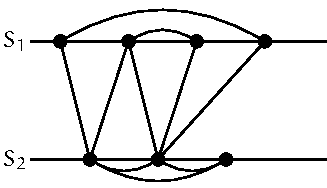
\includegraphics{figures/t_two_spines}
    \caption[Two-spine drawing]{A two-spine drawing.}
    \label{figure:two_spines}
\end{figure}

We now consider another variation on book embedding which 
will turn out to be a special case of the latter application of \PQ-trees.
It is a generalisation of the 2-page case that uses not just one spine but several parallel
spines~(lines) $S_1$, \dots, $S_k$. In the following considerations we always assume
that $S_i$~is above~$S_{i+1}$ for all $i\in\range{k-1}$.
We want to planarly draw one graph above~$S_1$,
one between~$S_i$ and $S_{i+1}$ for each $i \in \range{k-1}$ and one
below~$S_k$, as depicted in \myref{figure:two_spines} for
two spines. This problem is motivated by \emph{level planarity} which
is the same problem without the \emph{caps}, the graph above~$S_1$ and
the graph below~$S_k$.
The level planarity problem was first introduced by Tomii~et.~al.~\cite{Tomii77}. 
Jünger, Leipert and
Mutzel presented an algorithm that checks for level planarity in linear time~\cite{Junger99}.

In this section we show that the multiple spine problem is equivalent to a 2-page book embedding problem constrained by a special \PT-tree, but do not manage to give an efficient algorithm
it. Still, this reinforces our belief that \probPTree is an interesting problem.

Let the spines always be~$S_i = \SR \times \{-i\}$. We now formally define
the problem. It will turn out to be convenient to formally use directed edges pointing downward for the edges between the spines, but we still understand and draw these edges as undirected edges.

\newProb{\probMul}{Vertex sets~$V_1$, \dots, $V_k$ and
edge sets $E_0 \subseteq \binom{V_1}{2}$, $E_1 \subseteq V_1\times V_2$,
\dots, $E_{k-1} \subseteq V_{k-1} \times V_k$, $E_k \subseteq \binom{V_k}{2}$.}{Is there
a planar drawing of $(V_1 \cup \dotsb \cup V_k, E_0 \cup \dotsb \cup E_k)$ such that
a vertex in~$V_i$ lies on~$S_i$ for all~$i \in \range{k}$, edges do not cross a spine,
the edges in~$E_0$ lie completely above~$S_1$ and the edges in~$E_k$ lie completely below~$S_k$?}

Tomii~et.~al.~\cite{Tomii77} showed that the 2-level planar graphs are exactly the forests
of caterpillars. Recall that a \emph{caterpillar} is a tree all of whose vertices are on
a central path or one edge away from it. Therefore, each of the graphs~$(V_i \cup V_{i+1}, E_i)$ for~$i \in \range{k-1}$ has to be a forest, \ie we find~$|E_i| = |V_i| + |V_{i+1}| - l$ if this
forest has $l$~components. That is, as in the case of page embedding the number of edges is again linear in
the number of vertices. Thus, the size of a \probMul~instance is in~$\OO\bigl(|V_1| + \dotsb + |V_k|\bigr)$.

\begin{figure}[\placement]\centering
    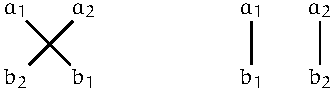
\includegraphics{figures/t_level_order}
    \caption[Level planarity is an ordering problem]{Level planarity only depends on the order of the vertices.}
    \label{figure:level_order}
\end{figure}

From \myref{lemma:constraints} we know that book embedding is essentially an ordering problem.
Similarly, consider two edges $(a_1, b_1)$ and~$(a_2, b_2)$ lying between the same two spines
and investigate how their embeddability depends on the order of their endpoints. If
$a_1$~lies left of~$a_2$ on the upper spine and $b_2$~lies left of~$b_1$ on the lower spine, then any Jordan curve from $a_1$ to~$b_1$ between the spines must intersect with any Jordan curve from $a_2$ to~$b_2$ between the spines by the Jordan curve theorem, \ie there cannot 
be a level embedding with this order. This case is depicted in \myref{figure:level_order}. Similarly,
if $a_2$~lies left of~$a_1$ and $b_1$~lies left of~$b_2$, the edges~$(a_1, b_1)$ and~$(a_2, b_2)$ also
cannot be embedded.

In any other order we can just draw a straight line for both
edges to obtain a valid embedding of the edges. After combining these observations for all pairs
of edges and taking the caps into account, we get a total order formulation of \probMul.
 
\begin{lemma}\label{lemma:multi_spine_total}
Let~$I := (V_1, \dotsc, V_k, E_0, \dotsc, E_k)$ be a \probMul instance. Then~$I$ is solvable
if any only if there is a linear order~$<_i$ on~$V_i$ for each $i \in \range{k}$ such
that the following properties hold. For all~$i \in \{1, \dots, k-1\}$ and pairs of edges~$(a_1, b_1), (a_2, b_2) \in E_i$ the order $a_1 <_i a_2 \land b_2 <_{i+1} b_1$ does not occur. Furthermore,
for $i\in\{0, k\}$ and all $\{a, b\}, \{c, d\} \in E_i$ we must not have $a <_i c <_i b <_i d$.
\end{lemma}

The order constraint for level planarity looks very similar to the book constraint,
just separated into two total orders. Indeed, if we have a \probMul instance we can find a corresponding
book embedding instance.
\begin{figure}\centering
    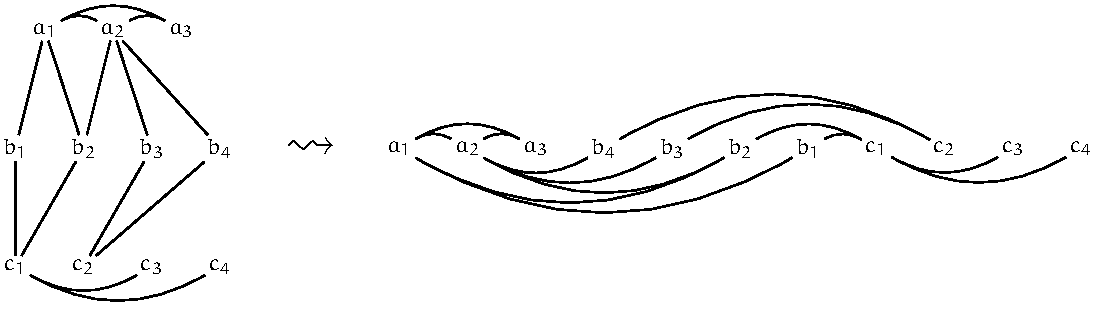
\includegraphics[width=0.9\textwidth]{figures/t_level_map}
    \caption[\probMul instance to book embedding instance]{A \probMul instance can be transformed into a 2-page book embedding instance
with separated sets of vertices.}
    \label{figure:level_map}
\end{figure}
\vskip1em
\begin{theorem}
Let~$I := (V_1, \dotsc, V_k, E_0, \dotsc, E_k)$ be a \probMul instance. We define
a corresponding 2-page book embedding instance by taking $V := V_1 \cup \dotsb \cup V_k$
as vertices and 
\begin{align*}
\widetilde{E}_1 := \bigcup_{\substack{i \in \{0, \dotsc, k\}\\ i \text{\emph{ even}}}} E_i\\
\widetilde{E}_2 := \bigcup_{\substack{i \in \{0, \dotsc, k\}\\ i \text{\emph{ odd}}}} E_i
\end{align*}
as pages. Then~$I$ is solvable if and only if~$J := (V, \widetilde{E}_1, \widetilde{E}_2)$
has a book embedding where the vertices in each~$V_i$ are consecutive.
\end{theorem}

\begin{myproof}
\begin{itemize}
\item[]
\item[``$\Rightarrow$''] Let~$<_i$ for~$i \in \range{k}$ be total orders forming a valid 
embedding of~$I$. 

Then define~$<$ on~$V$ to be the total order that first lists the
vertices of~$V_1$, then the vertices of~$V_2$, and so on. Get the inner order of the vertices
in~$V_i$ from~$<_i$ if~$i$ is even and from~$<_i$ reversed if~$i$ is odd. This
construction is illustrated in \myref{figure:level_map}.

The order~$<$ is a valid solution of the book embedding problem~$J$:
The edges in distinct edge sets~$E_i$ do not intersect by the construction of~$<$ and the definitions
of $\widetilde{E}_1$ and $\widetilde{E}_2$. Edges in~$E_0$ or~$E_k$ do not intersect since~$<_1$
and~$<_k$ are valid page embeddings for~$(V_1, E_0)$ and~$(V_k, E_k)$, respectively. Now take
two edges~$(a_1, b_1), (a_2, b_2) \in E_i$ for some~$i \in \range{k-1}$. If~$a_1 < a_2 < b_1 < b_2$
occurs, we have~$a_1 <_i a_2\;\land\;b_1 <_{i+1} b_2$, contradicting the validity of
the initial solution of~$I$. Thus, the book constraint for the two edges is fulfilled.
\item[``$\Leftarrow$''] Let~$<$ be a valid book order of~$J$ where
the sets~$V_i$ with~$i \in \range{k}$ are separated. Do the construction above in reverse, \ie
define~$<_i$ to be the restriction of~$<$ to~$V_i$ for all~$i \in \range{k}$. Additionally,
reverse~$<_i$ when~$i$ is odd.

The order~$<_i$ yields a valid embedding for~$I$: The caps already appeared in the book embedding
problem~$J$, \ie they are still valid. If~$a_1 <_i a_2\;\land\;b_2 <_{i+1} b_1$ occurs for some~$(a_1, b_1), (a_2, b_2) \in E_i$ and~$i \in \range{k-1}$, then we must have either~$a_1 < a_2 < b_1 < b_2$,
$a_2 < a_1 < b_2 < b_1$, $b_1 < b_2 < a_2 < a_1$ or~$b_2 < b_1 < a_1 < a_2$. All of these
cases contradict the book constraints.\qedhere
\end{itemize}
\end{myproof}

\paragraph{Outlook}

All in all, we see that \probMul is equivalent to a 2-page book
embedding problem where the vertex sets~$V_i$ with~$i \in \range{k}$ have to be 
separated. This separation can be modelled by a \PT-tree by introducing a \PT-node
connected to the vertices~$V_i$ for all~$i \in \range{k}$ and connecting all 
of these \PT-nodes to a single root. 

Since \probMul is an interesting problem in its own right, this leaves several
distinct possibilities for further results:
\begin{itemize}
\item Provide a polynomial time algorithm for  \probPTree and get an efficient solution of \probMul.
\item Prove the \NP-completeness of \probMul and get the \NP-completeness of \probPTree.
\item Provide a polynomial time algorithm for \probMul and get an efficient algorithm for a special case of \probPTree.
\end{itemize}